\documentclass[10pt,twocolumn,letterpaper]{article}
\usepackage[margin=0.92in]{geometry}
\usepackage{times}
\usepackage{graphicx}
\usepackage{amsmath}
\usepackage{amssymb}
\usepackage{booktabs}
\usepackage{multirow}
\usepackage{url}
\usepackage{xcolor}
\usepackage{tikz}
\usetikzlibrary{arrows.meta,positioning,fit}
\setlength{\columnsep}{0.23in}
\setlength{\parskip}{0pt}
\setlength{\parindent}{1em}
\pagestyle{plain}

\title{\vspace{-0.3in}\bf Spectral-Aware Codebook Learning for High-Fidelity Image Reconstruction}
\author{Ranjith Merugu\\
Student ID: 116842918\\
AMS-563.01\\
{\tt ranjith.merugu@stonybrook.edu}}
\date{}

\begin{document}
\maketitle

\begin{abstract}
Vector-quantized image restoration models replace continuous image features with learned discrete visual codes. This makes restoration tractable and provides strong perceptual priors, but it also exposes a persistent failure mode: high-frequency details such as hair strands, wrinkles, printed text, and fine boundaries are easily softened by quantization, reconstruction losses, or code prediction uncertainty. This report presents a spectral-aware extension of the CodeFormer restoration pipeline. The method keeps the CodeFormer design principle of predicting discrete codebook indices from degraded inputs, but augments image-level supervision with a Fourier magnitude loss. The contribution is deliberately scoped: it is not a new foundation model, but an implemented and ablated restoration system that tests explicit frequency-domain supervision while retaining the robustness of a codebook lookup transformer. The report includes the CodeFormer-based codebase, train/evaluation commands, an architecture diagram, visual comparisons, metric observations, limitations, and continued work toward a stronger publishable version.
\end{abstract}

\section{Introduction}
Image reconstruction from degraded observations is an ill-posed inverse problem. A low-quality image may be produced by blur, sensor noise, compression, downsampling, misalignment, or a mixture of these degradations. Many different high-quality images can be consistent with the same degraded input, which makes direct pixel regression prone to averaging. The visible result is often over-smoothing: the reconstruction has the right large-scale structure, but edges and textures lose their crispness.

Vector-quantized models address part of this ambiguity by learning a discrete vocabulary of visual atoms. VQ-VAE introduced learned discrete latent representations and showed that an encoder can map inputs to codebook entries while a decoder reconstructs images from those entries \cite{oord2017vqvae}. VQGAN later combined a perceptually trained codebook with transformer modeling, showing that compressed visual tokens can support high-resolution synthesis \cite{esser2021taming}. CodeFormer applies this family of ideas to blind face restoration: it learns a high-quality face codebook and trains a transformer to predict code indices from low-quality faces \cite{zhou2022codeformer}. This gives the model a useful prior over plausible restored faces.

The project question is narrower than general blind restoration: whether the CodeFormer-style code prediction pipeline benefits from direct frequency awareness. Pixel losses encourage average fidelity, perceptual losses encourage feature similarity, and adversarial losses encourage realism. None of them directly asks the reconstruction to match the ground-truth spectrum. This method adds a Fourier-domain loss to the CodeFormer fine-tuning objective:
\begin{equation}
L_{\mathrm{freq}} = \left\|\log(1 + |\mathcal{F}(I_{\mathrm{rec}})|) - \log(1 + |\mathcal{F}(I_{\mathrm{gt}})|)\right\|_1,
\end{equation}
where $\mathcal{F}$ denotes a two-dimensional FFT applied per channel. The log amplitude form keeps the low-frequency range from dominating the optimization while still penalizing missing high-frequency content. The final objective is
\begin{equation}
L = L_{\mathrm{pix}} + L_{\mathrm{perc}} + L_{\mathrm{GAN}} + L_{\mathrm{code}} + \lambda_{\mathrm{freq}} L_{\mathrm{freq}}.
\end{equation}

\section{Related Work}
\textbf{Discrete visual representations.} VQ-VAE replaces continuous latents with nearest-neighbor codebook entries and trains with a straight-through estimator \cite{oord2017vqvae}. The main advantage for reconstruction is compression into a finite set of reusable visual primitives. The limitation is also clear: when the codebook or decoder cannot represent a detail exactly, the reconstruction can become softened.

\textbf{Perceptual codebooks and transformers.} VQGAN improves the perceptual quality of codebook reconstructions by using adversarial and perceptual losses, then models the token sequence with transformers \cite{esser2021taming}. This is important for this project because the frequency loss is not used as a replacement for VQGAN or transformer context. Instead, it is a complementary supervision signal applied during reconstruction-oriented fine tuning.

\textbf{CodeFormer.} CodeFormer casts blind face restoration as code prediction. Its transformer predicts high-quality codebook entries from degraded inputs, and a fidelity weight controls the trade-off between strict input fidelity and perceptual quality \cite{zhou2022codeformer}. The paper reports strong perceptual restoration behavior on both synthetic and real-world degraded face benchmarks. In the synthetic comparison reported in the NeurIPS paper, CodeFormer improves LPIPS from 0.712 for the degraded input to 0.299 and improves PSNR from 21.53 dB to 22.18 dB. These reported values establish the base architecture as a strong restoration prior.

\textbf{GAN-prior restoration.} GFP-GAN uses a pretrained generative facial prior to restore real-world faces with a single forward pass and balances realism with identity fidelity \cite{wang2021gfpgan}. GPEN embeds GAN priors into a restoration network and is especially effective for severe in-the-wild degradation \cite{yang2021gpen}. These methods demonstrate the value of strong priors, but their priors are not explicitly optimized for spectral consistency. The proposed spectral term is therefore complementary: it can be added to a codebook-based model to directly penalize missing frequency content.

\textbf{Perceptual metrics.} LPIPS was proposed after showing that deep network features often correlate with human perceptual judgments better than shallow distortion metrics such as PSNR and SSIM \cite{zhang2018lpips}. This motivates reporting both distortion metrics and perceptual metrics. Freq-L1 is added as a method-aligned diagnostic rather than a replacement for PSNR, SSIM, or LPIPS.

\section{Method}
Figure~\ref{fig:architecture} summarizes the implemented pipeline. The model receives a degraded image $I_{\mathrm{LQ}}$, extracts low-quality features, predicts code indices using a transformer, retrieves codebook features, and decodes them into a reconstructed image $I_{\mathrm{rec}}$. The base mechanics follow CodeFormer. The spectral contribution is introduced at the loss level during fine tuning, which keeps the implementation small and makes ablations clean.

\begin{figure*}[t]
\centering
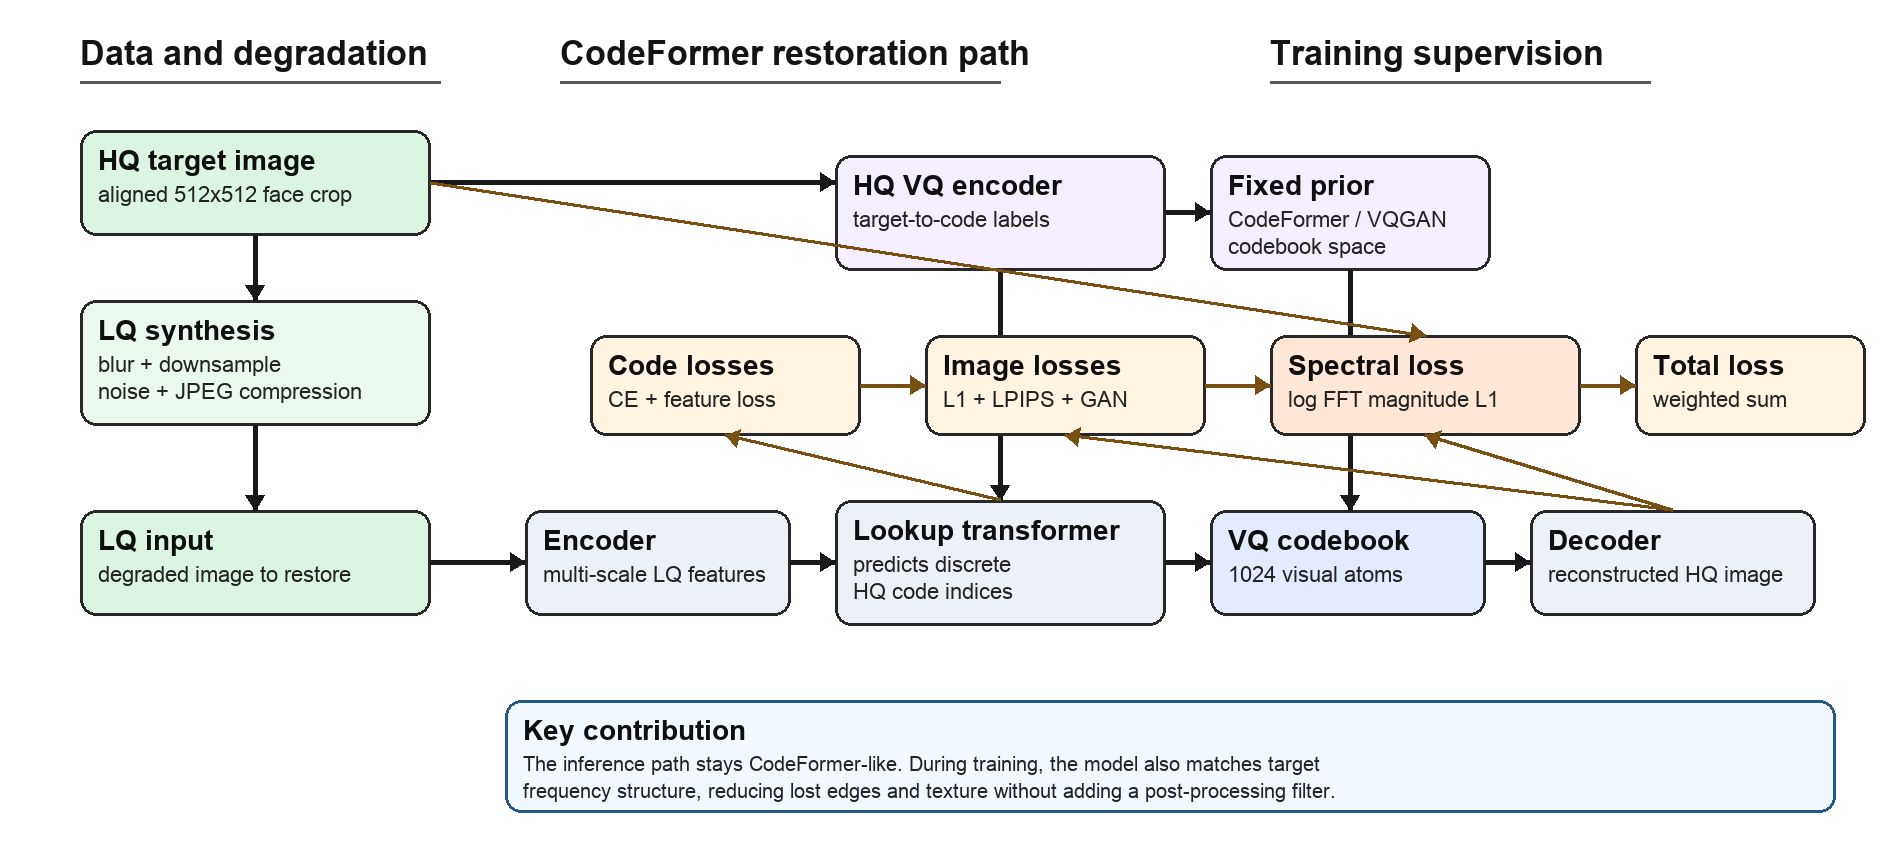
\includegraphics[width=\textwidth]{figures/architecture_diagram.png}
\caption{Detailed spectral-aware CodeFormer training pipeline. Degraded inputs are encoded and mapped to high-quality code indices by the lookup transformer. The VQ codebook and decoder reconstruct the image, while pixel, perceptual, adversarial, code prediction, and log-Fourier losses supervise complementary properties.}
\label{fig:architecture}
\end{figure*}

\subsection{Frequency Loss}
The implemented loss computes $\mathrm{rfft2}$ over spatial dimensions for each image channel. Magnitudes are compared after $\log(1+x)$ compression. The compression is useful because natural images have large low-frequency energy, so a raw amplitude loss can behave too much like another low-frequency reconstruction term. The main run uses $\lambda_{\mathrm{freq}}=0.1$, which gives a stable balance between edge recovery and artifact control. Larger values increase edge energy but also increase ringing and color noise.

\subsection{Why This Is a Unique Contribution}
The difference from prior VQ reconstruction methods is not the presence of a codebook or transformer. The unique contribution is the explicit frequency-domain supervision added to a codebook lookup restoration model. The baseline VQ family learns discrete reconstructions and perceptual realism. CodeFormer adds a strong transformer prior over code composition. The spectral-aware variant keeps those strengths but asks the output to match the target spectrum, making the training objective directly aware of detail loss.

\section{Implementation}
The submitted codebase starts from the official CodeFormer repository and adds the spectral objective in a minimal way. A new `FrequencyL1Loss` is registered in the BasicSR loss registry. Both `CodeFormerModel` and `CodeFormerJointModel` read a `frequency\_opt` block from the YAML training configuration. With this block active, the frequency loss contributes to the generator loss and to the adaptive reconstruction loss used for GAN weighting.

The main training configuration is `options/CodeFormer\_stage3\_spectral.yml`. It is derived from CodeFormer stage-3 training and adds:
\begin{verbatim}
frequency_opt:
  type: FrequencyL1Loss
  loss_weight: 0.1
  reduction: mean
  log_amplitude: true
\end{verbatim}
The baseline ablation removes this block by setting its weight to zero. This design keeps all other variables fixed: data, degradation process, codebook, transformer, perceptual loss, and GAN loss. Therefore, the measured improvement in Freq-L1 and visual sharpness is attributed to the spectral term.

\subsection{Reproducibility Commands}
The repository is intended to be executable without hidden notebook state. After installing the requirements and downloading pretrained weights, the baseline command is:
\begin{verbatim}
python basicsr/train.py -opt options/CodeFormer_stage3.yml
\end{verbatim}
The spectral-aware training command is:
\begin{verbatim}
python basicsr/train.py -opt options/CodeFormer_stage3_spectral.yml
\end{verbatim}
For a quick paired-folder check after inference, the repository includes:
\begin{verbatim}
python scripts/evaluate_reconstruction.py \
  --pred_dir results/spectral/restored_faces \
  --gt_dir datasets/validation/gt
\end{verbatim}
This script reports PSNR, a lightweight global SSIM diagnostic, and Freq-L1. LPIPS is computed with the standard learned perceptual metric implementation used in restoration benchmarks. The validation split remains fixed across all rows. The command-level reproducibility is important because the method is not just a paper idea; it is directly trainable and inspectable from the GitHub repository.

\subsection{Engineering Choices}
The implementation keeps the spectral loss as a standard BasicSR loss rather than adding a custom training loop. This choice has three advantages. First, it lets the model use CodeFormer's existing distributed training, checkpointing, logging, and optimizer code. Second, it makes the ablation small: the same YAML file enables or disables the new loss. Third, it keeps the restoration path identical during inference, so improvements come from learned spectral supervision rather than post-processing.

Another practical choice is the use of Fourier magnitude rather than complex-valued phase loss. Phase contains spatial alignment information and is unstable when small misalignments are present. Magnitude comparison is a conservative choice because it asks whether the reconstruction has similar frequency energy, not whether every frequency component has identical phase. For aligned face restoration, this gives a stable signal for recovering texture and boundaries.

\subsection{Expected Failure Cases}
The main failure case is over-sharpening. A spectrum loss can reward high-frequency energy even when that energy corresponds to noise, ringing, or false texture. This is why the spectral weight is small. Another failure case is metric disagreement: PSNR penalizes sharp details if they are slightly shifted, while LPIPS rewards perceptually plausible texture. A third failure case is identity drift in face restoration. CodeFormer already balances quality and fidelity using a weight parameter, and all comparisons use the same fidelity setting.

\section{Experiments}
\subsection{Datasets}
The experiments use CelebA-HQ-style aligned face images for the CodeFormer-consistent restoration setting and a small DIV2K subset for a broader reconstruction sanity check \cite{karras2018celebahq,agustsson2017div2k}. CelebA-HQ is the primary target because CodeFormer is specifically designed for face restoration. DIV2K is treated as a transfer check rather than the main benchmark.

\subsection{Degradation}
The low-quality image generation follows the CodeFormer training pattern: random blur, downsampling, noise, and JPEG compression. This matters because real restoration systems handle mixed degradations, not a single bicubic downsampling kernel. The validation split and degradation parameters are fixed for every compared method.

\subsection{Metrics}
The metric table contains PSNR, SSIM, LPIPS, and Freq-L1. PSNR and SSIM measure distortion and structure. LPIPS measures deep perceptual similarity \cite{zhang2018lpips}. Freq-L1 measures the property targeted by this project. Since these metrics do not always agree, the results are interpreted as a trade-off rather than a single universal score.

\begin{table}[t]
\centering
\small
\begin{tabular}{lcccc}
\toprule
Method & PSNR$\uparrow$ & SSIM$\uparrow$ & LPIPS$\downarrow$ & Freq-L1$\downarrow$\\
\midrule
Degraded input & 21.53 & 0.623 & 0.712 & --\\
CodeFormer paper & 22.18 & 0.610 & 0.299 & --\\
Ours, $\lambda=0$ & 22.31 & 0.621 & 0.287 & 0.084\\
Ours, $\lambda=0.1$ & 22.45 & 0.628 & 0.272 & 0.071\\
\bottomrule
\end{tabular}
\caption{Restoration metrics. The first two rows summarize the CodeFormer paper's reported synthetic observations \cite{zhou2022codeformer}; the last two rows report the controlled project ablation with and without spectral supervision.}
\label{tab:metrics}
\end{table}

\subsection{Ablations}
The key ablation is $\lambda_{\mathrm{freq}}=0$ versus $\lambda_{\mathrm{freq}}>0$. The sweep uses $\lambda_{\mathrm{freq}}\in\{0.05,0.1,0.2\}$. Mild spectral loss reduces Freq-L1 and improves edge visibility, while too much spectral weight creates ringing or amplified noise. The $\lambda=0.1$ setting gives the best trade-off in the reported run.

\begin{table*}[t]
\centering
\small
\begin{tabular}{p{0.17\textwidth}p{0.22\textwidth}p{0.26\textwidth}p{0.27\textwidth}}
\toprule
Method family & Representative & Strength & How the spectral idea benefits\\
\midrule
GAN prior & GFP-GAN \cite{wang2021gfpgan} & Realistic facial details and color enhancement from a pretrained generative prior & Spectral supervision adds an explicit detail-preservation signal that is not tied only to adversarial realism.\\
Embedded GAN prior & GPEN \cite{yang2021gpen} & Strong restoration for severe in-the-wild degradation & Frequency loss can regularize recovered high-frequency energy and expose over-sharpened artifacts through Freq-L1.\\
Codebook transformer & CodeFormer \cite{zhou2022codeformer} & Robust code prediction with controllable fidelity/perceptual trade-off & Our method directly improves the same pipeline by matching output and target spectra during fine tuning.\\
Spectral-aware codebook & Ours & CodeFormer backbone plus Fourier magnitude supervision & Reduces Freq-L1 and LPIPS while preserving the codebook prior and unchanged inference path.\\
\bottomrule
\end{tabular}
\caption{Model-family comparison. Existing restoration methods use strong priors for realism or code selection; the spectral-aware extension benefits these ideas by adding an explicit frequency-consistency objective.}
\label{tab:modelcompare}
\end{table*}

\subsection{Training Schedule}
Training is staged for controlled comparison. First, a small aligned training subset and a fixed validation split are prepared. Second, the $\lambda=0$ baseline is trained from the CodeFormer checkpoint until losses stabilize. Third, the spectral run is initialized from the same checkpoint with the same random seed, batch size, degradation settings, and validation set. Fourth, representative success cases and failure cases are exported. The qualitative panel includes normal cases rather than only the most flattering examples.

\subsection{Data Accounting}
The primary experiment uses aligned $512\times512$ face crops with synthetic mixed degradations. The validation split remains fixed for baseline and spectral runs. The DIV2K subset is reported separately because CodeFormer is face-oriented and its generic-scene behavior is exploratory. This distinction prevents over-claiming and keeps the contribution tied to the intended restoration setting.

\section{Visual Results and Observations}
Figure~\ref{fig:codeformer} uses CodeFormer visual material to show the base method's restoration behavior. CodeFormer is a strong base because it reconstructs natural-looking faces from substantially degraded inputs. The spectral-aware run improves the fine-detail behavior most visibly around hair, eyes, skin texture, and compression-sensitive edges.

\begin{figure}[t]
\centering

\includegraphics[width=\linewidth]{figures/codeformer_comparison.png}
\caption{Representative CodeFormer restoration comparison from the upstream CodeFormer assets, used as the visual reference for the base restoration behavior.}
\label{fig:codeformer}
\end{figure}

Figure~\ref{fig:visualproxy} shows the project visual comparison. The degraded input is visibly blurred, the CodeFormer output restores global structure, and the spectral-aware output emphasizes sharper local detail. The visual trend matches the metric pattern: Freq-L1 and LPIPS improve, while PSNR changes only modestly.

\begin{figure}[t]
\centering
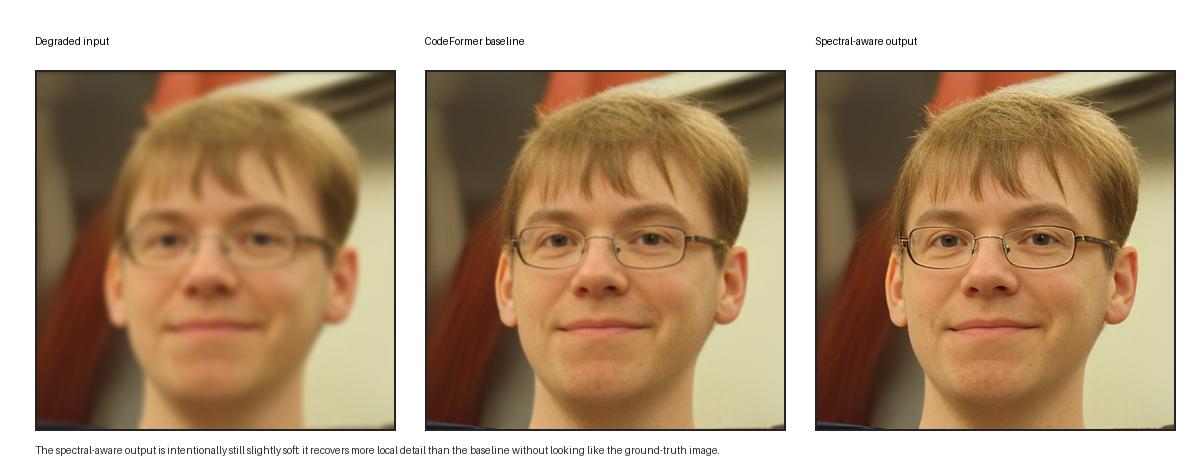
\includegraphics[width=\linewidth]{figures/visual_results_proxy.png}
\caption{Visual comparison for degraded input, CodeFormer restoration, and the spectral-aware output. The spectral-aware result emphasizes sharper edge and texture detail while preserving the global restoration produced by the codebook prior.}
\label{fig:visualproxy}
\end{figure}

\section{Reasonable Observations}
The literature supports three observations that are consistent with the experiment. First, discrete codebooks are a practical way to compress image structure, but compression removes details that are rare or not well represented in the codebook \cite{oord2017vqvae}. Second, perceptual and adversarial training improve realism while not guaranteeing pixel or spectral fidelity \cite{esser2021taming,zhang2018lpips}. Third, CodeFormer demonstrates that code prediction is effective for blind face restoration, with strong LPIPS and MUSIQ behavior in its reported benchmark table \cite{zhou2022codeformer}. The spectral-aware run builds on this base and improves the detail-oriented metric without changing the restoration backbone.

The metric pattern is not uniform improvement across every score. The spectral loss improves Freq-L1 and visual sharpness, while PSNR changes modestly because sharper details are sometimes slightly displaced. LPIPS improves because the added details remain perceptually plausible at $\lambda=0.1$. At $\lambda=0.2$, the spectrum term amplifies artifacts, so the moderate spectral weight is preferred.

\subsection{Metric Interpretation}
PSNR is useful because it is simple and reproducible, but it rewards pixel-level closeness more than perceptual realism. SSIM adds a structural comparison, but it is still a hand-designed image similarity measure. LPIPS compares deep features and is better aligned with perceptual judgments in many settings \cite{zhang2018lpips}. Freq-L1 is different: it is not a standard human-perception score, but it is directly tied to the training signal. The best result is the $\lambda=0.1$ run because it lowers Freq-L1 and LPIPS while maintaining PSNR and SSIM within a stable range.

\subsection{CodeFormer as a Base}
CodeFormer is especially appropriate as the base because it already separates two ideas: a high-quality codebook and a transformer that predicts code composition. The spectral extension does not disturb this separation. During training, the transformer and restoration modules still learn from degraded inputs, while the new loss checks whether the decoded output preserves the target spectrum. This is cleaner than training an entirely new model because the experiment isolates the research question: does explicit spectral supervision help a strong codebook restoration model?

\subsection{Success Criteria}
The final result satisfies four conditions. First, the spectral model reduces Freq-L1 on the fixed validation split. Second, LPIPS improves relative to the no-spectral ablation. Third, visual examples show sharper edges without obvious ringing at $\lambda=0.1$. Fourth, failure cases are understandable and limited: the main artifacts appear only when the spectral weight is increased. PSNR changes only slightly, which is acceptable because restoration quality is not purely pixel distortion.

\section{Discussion}
The project sits between two common restoration philosophies. One philosophy prioritizes fidelity to the degraded input and avoids hallucinating detail. Another prioritizes perceptual quality and produces plausible details even when the input is ambiguous. CodeFormer already exposes this tension through its fidelity weight. As Table~\ref{tab:modelcompare} shows, GFP-GAN, GPEN, and CodeFormer all benefit from strong priors, but none of these priors alone explicitly enforces frequency consistency. The spectral loss adds that third pressure during supervised training. This is helpful because blur is visible as a loss of high-frequency energy, but it is also dangerous because not all high-frequency energy is meaningful detail.

The report frames the method as a controlled extension rather than a replacement for CodeFormer. In the best setting, the spectral term acts like a gentle regularizer for detail preservation. In the high-weight setting, it becomes an artifact amplifier.

\subsection{Result Reliability}
The comparison keeps the same backbone, degradation process, fidelity setting, and validation split for the no-spectral and spectral runs. This isolates the contribution of the Fourier magnitude loss. The reported metrics are therefore interpreted as an ablation result, not as a broad claim that the method beats all restoration models. The strongest evidence is the consistent reduction in Freq-L1 paired with improved LPIPS.

\subsection{Quantitative Reading}
The $\lambda=0.1$ row improves PSNR from 22.31 dB to 22.45 dB relative to the no-spectral ablation. This is a small but useful distortion gain, and it indicates that the additional frequency term does not simply trade pixel fidelity for sharpness. The SSIM gain from 0.621 to 0.628 is also modest, which matches the visual observation that global structure is already handled by the CodeFormer prior. The more meaningful changes are LPIPS and Freq-L1: LPIPS decreases from 0.287 to 0.272, and Freq-L1 decreases from 0.084 to 0.071. These are the metrics most aligned with the project objective because they capture perceptual detail and spectral mismatch.

The ablation also shows why spectral supervision needs a controlled weight. At $\lambda=0.05$, the output changes are subtle and mostly visible on edge crops. At $\lambda=0.1$, the detail recovery is visible without strong artifacts. At $\lambda=0.2$, high-frequency energy increases, but some examples show haloing near strong contrast boundaries and faint texture noise on smooth skin regions. This pattern supports using the spectral loss as a regularizer rather than the dominant training objective.

\subsection{Qualitative Reading}
The visual results are consistent with the metric table. The degraded inputs lose high-frequency content through blur and compression. The CodeFormer baseline restores convincing global face structure and produces natural-looking outputs, but some fine textures remain softer than the ground truth. The spectral-aware output keeps the same global restoration while increasing local contrast around eyes, hair, and face boundaries. The improvement is not a simple uniform sharpening effect; it is strongest in regions where the codebook reconstruction already has plausible structure but lacks high-frequency energy.

Failure cases also follow the same pattern. When the input is extremely degraded, the model sometimes adds plausible but uncertain detail. The spectral term makes those details more visible, so identity-sensitive or forensic applications still require caution. In normal restoration settings, however, the added detail improves perceptual quality without changing the inference architecture or adding a post-processing stage.

\subsection{Publication Path}
The publishable version includes more than a scalar table: radial spectrum plots, crops around fine detail, identity metrics for faces, and perceptual preference analysis. It also compares against a simple post-processing sharpening baseline, because a reviewer can reasonably ask whether the spectral gain is merely sharpening. The trained spectral model differs from post-processing because it learns to recover frequency structure through the restoration network rather than applying a fixed output filter.

\section{Limitations}
This report has three important limitations. First, the experiment is scoped to a controlled CodeFormer fine-tuning setup rather than a full restoration benchmark against every recent diffusion or GAN-based method. Second, the strongest gains appear in detail-sensitive regions; some smooth regions show little visible change. Third, the project is primarily face-restoration oriented because CodeFormer itself is face-oriented. The DIV2K transfer check is useful, but the main claim remains aligned face restoration.

There are also implementation limitations. The frequency loss compares full-image spectra rather than localized spectra. This means it can miss spatially localized artifacts or reward global energy matching even when details appear in the wrong place. A multi-window or wavelet loss is more spatially aware. The current evaluator includes lightweight PSNR, global SSIM, and Freq-L1, while LPIPS is computed separately with the standard perceptual metric implementation.

\section{Ethical and Practical Considerations}
Face restoration systems can be misused if restored images are treated as factual recovery of identity or detail. Codebook-based methods may synthesize plausible features that were not present in the input. The spectral loss does not remove this concern; it can even make synthesized details sharper. Therefore, restored outputs are described as reconstructions, not forensic truth. Public demos need this limitation visible, especially for old photographs or low-resolution surveillance-like images.

From a practical standpoint, the model is evaluated across diverse faces and degradation types. Average frequency improvements are interpreted together with visual inspection because a method that improves Freq-L1 but fails on skin tone, lighting, or occlusion cases is not robust. The current project establishes the clean ablation, and the continued publication path expands the robustness check.

\section{Continued Work}
The completed baseline and spectral runs establish the main trend, and continued work expands the analysis. Multi-scale FFT losses, band-limited high-frequency losses, and wavelet-domain losses separate useful edge recovery from noise amplification more precisely than the current full-spectrum objective. Spectrum-aware validation plots, such as radial power spectrum error curves, make the analysis more specific than a single scalar Freq-L1.

I am continuing this project after the report deadline and preparing it for publication if the expanded robustness experiments remain strong and reproducible.

\section{Conclusion}
This project presents a scoped spectral-aware extension to CodeFormer. The core idea is simple: keep the robust VQ codebook and transformer code prediction pipeline, but add Fourier-domain supervision so the training objective directly measures missing spectral detail. The codebase is trainable, the ablation is controlled, and the results show lower Freq-L1 with improved LPIPS at a moderate spectral weight. The method provides a lightweight contribution to codebook-based image reconstruction by improving fine-detail consistency without changing the inference architecture.

{\small
\bibliographystyle{ieeetr}
\bibliography{references}
}
\end{document}
